\chapter{Búsqueda de SUSY con fotones y Higgs en el estado final con producción fuerte}
% \addcontentsline{toc}{chapter}{Búsqueda de SUSY con fotones y Higgs en el estado final}
\chaptermark{Búsqueda de SUSY con fotones y Higgs en el estado final con producción fuerte}


% / Tesis lic / %
% El análisis para el cual está orientada esta Tesis consiste en la búsqueda de Supersimetría en eventos con un fotón aislado muy energético, jets y gran cantidad de energía faltante en estado final \cite{Alonso:2147473,ATLAS:2016fks,Collaboration:2198651}. La estrategia general de la búsqueda consiste en el conteo del número de eventos observado en exceso sobre el SM en una cierta región del espacio de observables rica en eventos de la señal considerada.


El trabajo realizado en esta Tesis se centra en la búsqueda de Supersimetría en eventos con un fotón energético y aislado, jets y gran cantidad de energía faltante en el estado final. La estrategia general de la búsqueda consiste en el conteo del número de eventos observado en exceso sobre el SM en una cierta región del espacio de observables rica en eventos de la señal considerada, método descripto en la Sección \ref{sec:statistical}. El objetivo es poder discriminar de los datos observados aquellos que podrían ser producto de un proceso supersimétricos (señal) de aquellos producto de procesos del SM (fondo).


\section{Muestras de señal a partir de simulaciones de Monte Carlo}

El modelo supersimétrico que motiva a la presente búsqueda consiste en un modelo GGM, por lo tanto la LSP es el gravitino cuya masa será del orden de unos pocos eV. La NLSP es en este caso el neutralino más liviano, que va a consistir en un estado de gauge mezcla de bino y higgsino
% , lo que le permite acoplar a fotones y bosones de higgs
. En particular para esta Tesis se estudia el caso fenomenológico en el cual el neutralino más liviano decae en proporciones iguales a $\gamma+\gravino$ y a $h+\gravino$. Esto último es posible si se elige al parámetro $\mu<0$ que favorece el decaimiento al higgs, y reduce el decaimiento al bosón $Z$, en cuyo caso ya fue previamente estudiado por otros análisis \cite{tesis_fran, tesis_joaco}. Para la producción de partículas supersimétricas a partir de la colisión $pp$ se consideró inicialmente la producción de gluinos. La parte del análisis que comprende la producción electrodébil se describe en el Capítulo \ref{cap:analysis_EWK}. Los gluinos pueden decaer subsecuentemente en partículas más livianas, hasta llegar a las NLSP y luego a la LSP, produciendo jets a su paso y generando el estado final buscado. Una cadena de decaimiento típica de este modelo se puede observar en la Figura \ref{fig:phb_feyn}.

\begin{figure}
  \centering
  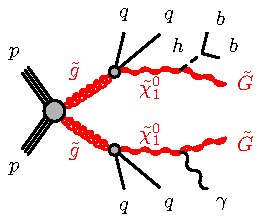
\includegraphics[width=0.5\textwidth]{images/analysis/gogo-qqqqbbphGG-h.pdf}
  \caption{Posible cadena de decaimiento del modelo supersimétrico en el que se centra esta Tesis.}
  \label{fig:phb_feyn}
\end{figure}

En la Sección \ref{sec:susy} se describe al MSSM juntos con la gran cantidad de parámetros que lo caracteriza. Cuando se desea generar muestras para un modelo, se debe elegir valores para esos parámetros que a priori son arbitrarios, y cuya única posible elección son los distintos objetivos del análisis. A su vez, se busca que al seleccionar valores para esos parámetros, tener el compromiso de no ser muy específicos con esos valores, ya que de esa forma el análisis terminaría siendo demasiado dedicado a un modelo particular. Ni tampoco muy arbitrarios, ya que se busca seguir manteniendo de alguna forma la fenomenología del mismo. Lo que se hace entonces es reducir los parámetros que caracterizan al modelo a unos pocos, y utilizar distintos programas de calculo que se encargan a partir de ellos generar tanto el espectro completo de masas, como los distintos posibles decaimientos de cada partícula.

El parámetro característico de este modelo es el $\mu$, el cual se elige negativo para habilitar el decaimiento del \ninoone a higgs. A su vez se desea anular el decaimiento al bosón $Z$, y que el decaimiento a fotones sea igual al de higgs, y para ello se eligió el valor óptimo de $M_1\sim -\mu$ \tosolve{Acá había encontrado una fórmula mediante un fit para M(mu), pero no se si es importante}. Con estos valores fue posible reducir el decaimiento al bosón $Z$ hasta casi un 10\%, dejando a los otros dos decaimientos aproximadamente en un 45\% como muestra la Figura \ref{fig:n1_br}. Como el modelo es un GGM, se fijó la masa del \gravino en $1$ eV \tosolve{esto no es tan así, la masa variaba de acuerdo al mu, lo deberia poner?}. 

\begin{figure}
  \centering
  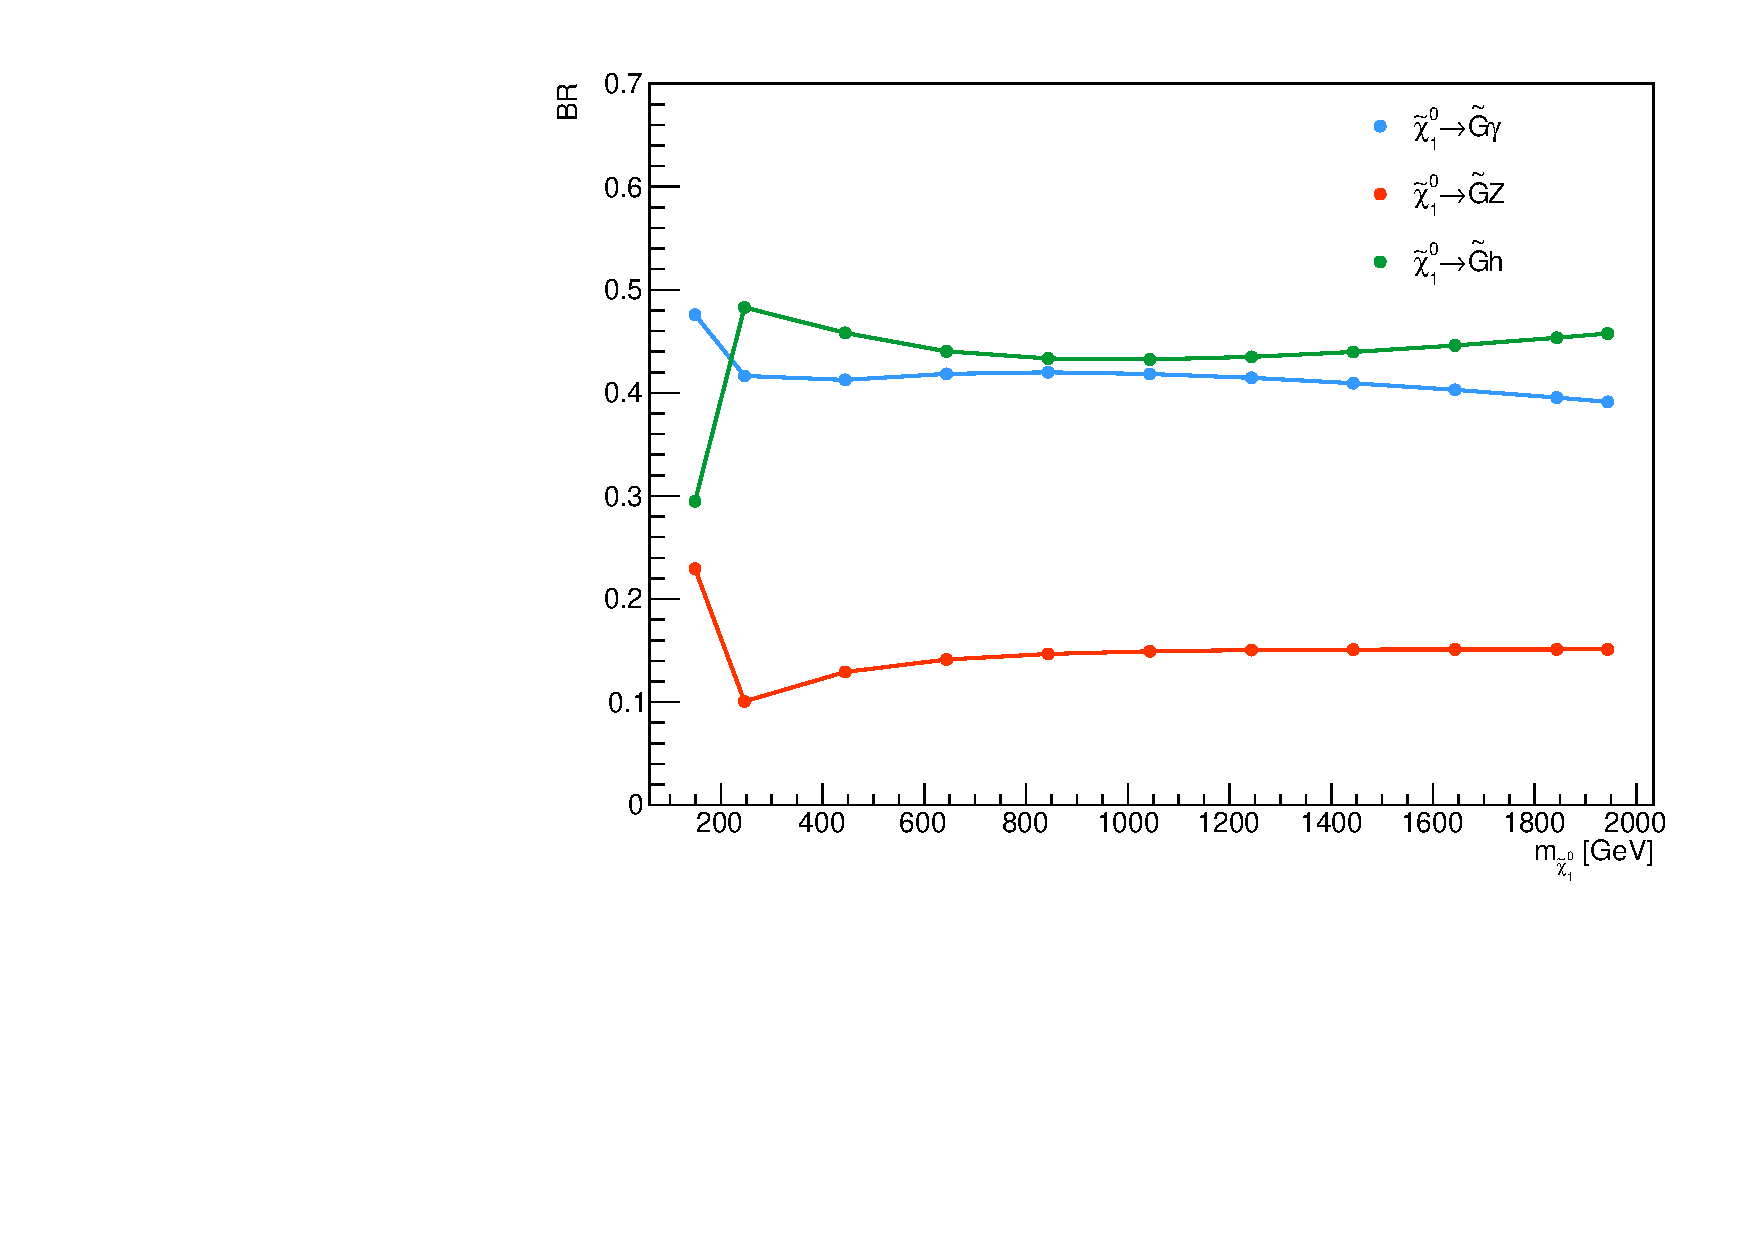
\includegraphics[width=0.6\textwidth]{images/analysis/phb_n1_br.pdf}
  \caption{Fracción de decaimiento del \ninoone en función de la masa del mismo.}
  \label{fig:n1_br}
\end{figure}

Las muestras fueron generadas considerando solamente la producción de gluinos a partir de la colisión $pp$. Además se eligió al gluino como la única partícula supersimétrica de color relevante, por lo que las masas de los squarks fueron fijadas a $5$ TeV, evitando así toda posible producción de los mismos. Los gluinos producidos en la colisión podían decaer un par de quark-antiquark más algún gaugino como se muestra en la Ecuación \ref{eq:gluino_dec}. Esto ocurre mediante squarks virtuales los cuales son completamente degenerados, pudiendo ser cualquiera de los 12 estados de sabor/quiralidad.

Además, se fijo a $M_2=3\ \tev$ y a $\tan{\beta}=1.5$ \tosolve{motivos formales?}. Todos los términos de acoplamiento trilineal fueron fijados a 0. Se eligió a la masa de los sleptons igual a $5$ TeV, para evitar así su producción la cual es estudiada por otros análisis. El bosón de higgs tiene una masa igual a la medida por las colaboraciones ATLAS y CMS \cite{higgs_mass}, $m_h=125\ \gev$, y sus decaimientos son elegidos de acuerdo a las predicciones del SM \tosolve{es asi?}, donde el predominante con un $\sim58$\% es a dos $b$-jets.
Adicionalmente se pone al mismo en el régimen de desacoplamiento con $m_A = 2\ \tev$. Al \ninoone se le fija su vida media, $c\tau_{\text{NLSP}}<0.1$ mm, de tal forma de que decaiga rápidamente  para que su vértice no esté muy desplazado del punto de colisión. Finalmente se anularon los decaimientos directos de los gluinos, charginos y neutralinos 1, 2 y 3. 

Debido a que son varios los análisis que estudian la producción de gluinos, la colaboración ATLAS puso a disposición unos archivos comunes a todos los análisis donde ya tiene almacenada la información de varios eventos de producción de gluinos. Estos archivos se denominan Les Houches Event (LHE), que le ahorran a cada análisis esta etapa de simulación, y sólo le resta generar las cadenas de decaimiento de los gluinos de acuerdo a sus modelos. En el presente análisis se omitieron correcciones radiativas así la masa de los los gluinos coincidía con el parámetro $M_3$, pudiendo así coincidir con los archivos LHE que están en función de la masa del mismo.

Los únicos parámetros libres del modelo son entonces $\mu$ y $M_3$ que determinan básicamente la masa de los \ninoone y gluinos. Se simularon 80 modelos distintos (puntos) con 10000 eventos en función de ambos parámetros, donde $150\ \gev<m_{\ninoone}<(m_{\tilde{g}}50)\ \gev$ y $1200\ \gev < m_{\tilde{g}}<2800\ \gev$. El arreglo completo de puntos de señal (grid) se puede observar en la Figura \ref{fig:grid_points}. Las muestras se realizaron con la simulación rápida del detector \textsc{ATLFAST-II} \tosolve{se supone que la voy a comentar en el segundo capitulo}. El espectro de masas completo, las fracciones de decaimiento de las sparticles y los anchos de decaimientos fueron calculados a partir del conjunto de parámetros anteriormente mencionados utilizando SUSPECT v2.43 \cite{Djouadi2007426}, SDECAY v1.5 \cite{Muhlleitner:2004mka} y HDECAY v3.4 \cite{Djouadi:1997yw}, que son parte del paquete SUSYHIT v1.5a \cite{Djouadi:2006bz}.
Como ejemplo se muestra en la Figura \ref{fig:mass_spec} un espectro de masas para unos de los puntos de señal con ($M_3$, $\mu$) = (1800 GeV, -1050 GeV). Un ejemplo de posibles decaimientos de los gluinos para ese mismo punto de señal se puede observar en la Figura \ref{fig:gluino_decays}. 

\begin{figure}
  \centering
  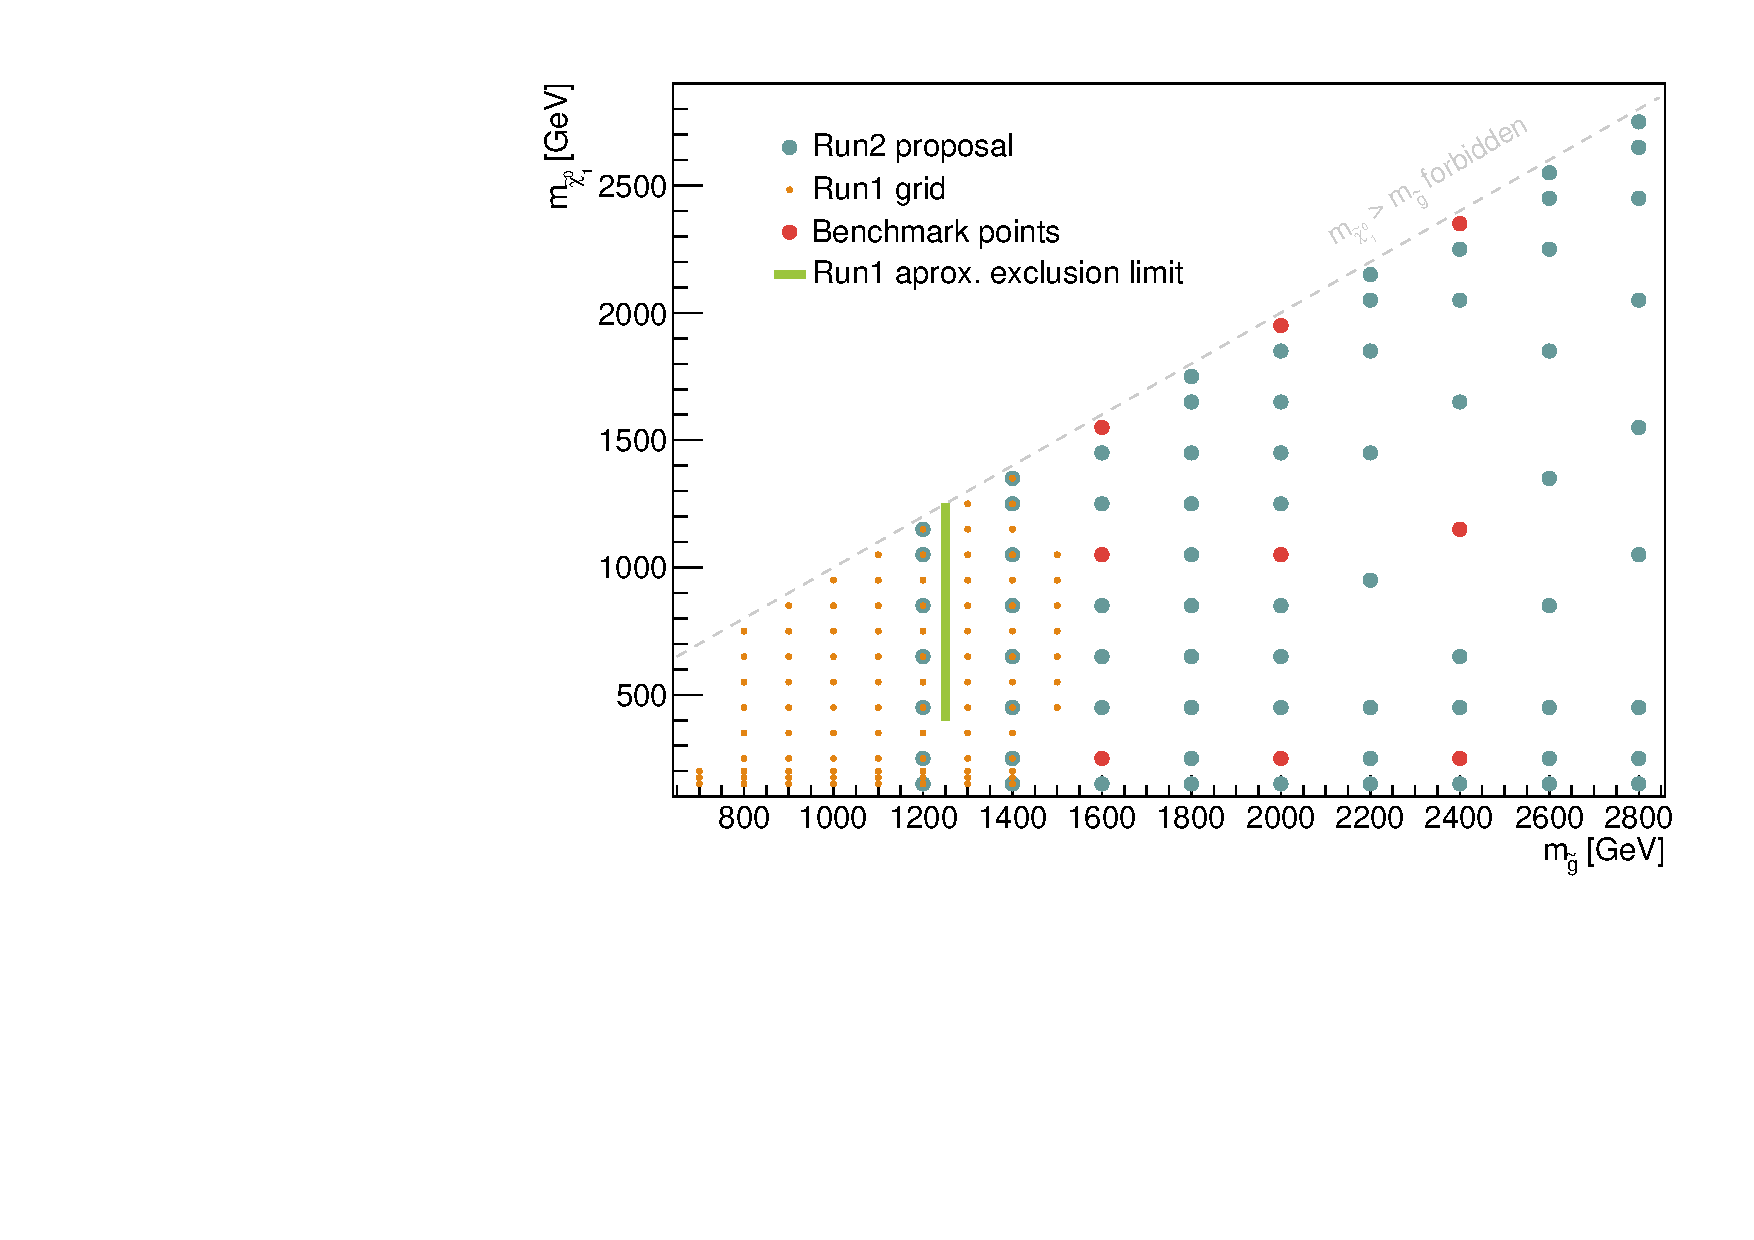
\includegraphics[width=0.6\textwidth]{images/analysis/phb_grid.pdf}
  \caption{Arreglo de muestras de señal generados en función de la masa del \ninoone y $\tilde{g}$. La densidad del mismo disminuye al aumentar $m_{\tilde{g}}$ debido a que la sensibilidad del análisis se estimó ser menor a los 2 TeV.}
  \label{fig:grid_points}
\end{figure}

\begin{figure}
  \centering
  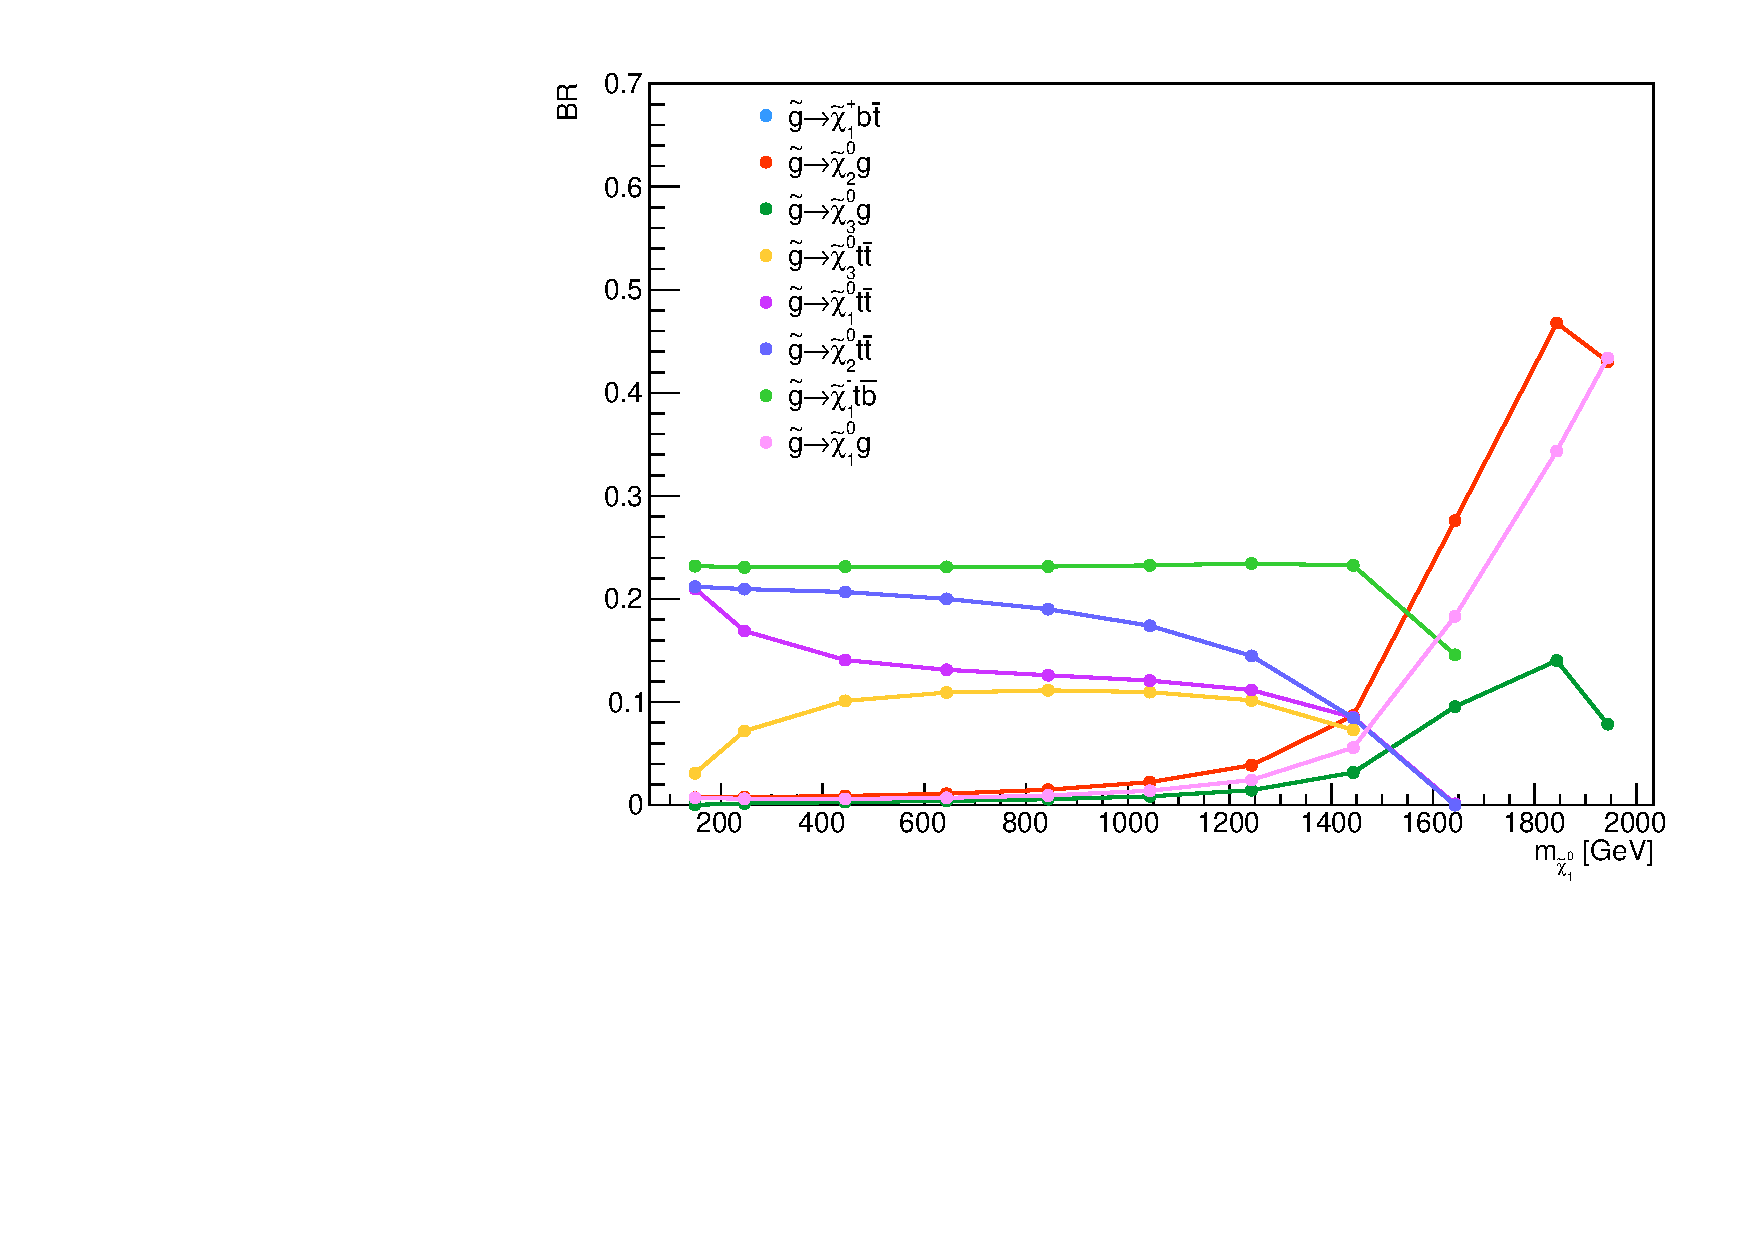
\includegraphics[width=0.6\textwidth]{images/analysis/phb_go_br.pdf}
  \caption{Fracción de decaimiento del gluino para el punto de señal con ($M_3$, $\mu$) = (1800 GeV, -1050 GeV). \tosolve{no sé si es necesario este plot...}}
  \label{fig:gluino_decays}
\end{figure}

\begin{figure}
  \centering
  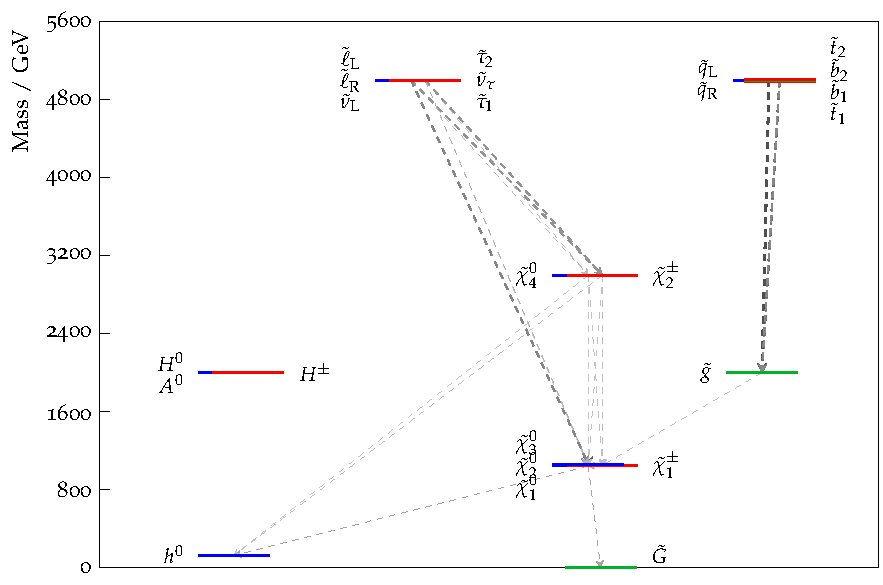
\includegraphics[width=0.6\textwidth]{images/analysis/phb_mass_spectrum.pdf}
  \caption{Espectro de masas de las sparticles para el punto de señal con ($M_3$, $\mu$) = (1800 GeV, -1050 GeV). \tosolve{hay una versión mejor de esta imagen}}
  \label{fig:mass_spec}
\end{figure}


\tosolve{Hay mas graficos de BR para poner, hacen falta? no lo creo...}

\section{Fondos del Modelo Estándar}


Los procesos del SM que son de interés como fondo para el análisis son aquellos que tienen un estado final igual al de la señal: fotones, jets y energía transversa faltante. Los mismos pueden clasificarse en distintos tipos. Por un lado, los procesos que dan lugar a eventos con un fotón y energía faltante real, es decir, los que se llaman fondos irreducibles. En este caso la energía la faltante proviene de los neutrinos, por lo que se componen principalmente de partículas que decaen a ellos, junto con fotones y jets de la ISR. Los procesos que cumplen con estos requisitos son la producción de bosones $Z$, $W$ y pares de top quarks que decaen subsecuentemente a bosones $W$:

\begin{itemize}
  \item $Z(\rightarrow \nu\nu) + \gamma + \text{jets}$
  \item $Z(\rightarrow \nu\nu) + \gamma + \gamma + \text{jets}$
  \item $W(\rightarrow l\nu) + \gamma + \text{jets}$
  \item $W(\rightarrow l\nu) + \gamma + \gamma + \text{jets}$
  \item $t\bar{t} + \gamma + \text{jets}$
\end{itemize}

Por otro lado es posible tener procesos que si bien no se producen fotones, unos de los objetos presentes en el mismo sea erróneamente reconstruido como tal, y genere un estado final igual al buscado pero con fotones `falsos'. Los objetos que pueden ser erróneamente reconstruidos como fotones en este caso pueden ser electrones o jets, por lo que hay que considerar aquellos procesos en los que se produzcan junto a neutrinos. Estos pueden ser:

\begin{itemize}
  \item $Z(\rightarrow \nu\nu) + \text{jets}$
  \item $W(\rightarrow l\nu) + \text{jets}$
  \item $t\bar{t} + \text{jets}$
\end{itemize}

Por último, puede ocurrir que si bien en el proceso no hayan neutrinos, una reconstrucción errónea de la energía de los distintos objetos presentes en el evento genere un desbalance a la hora de calcular la energía transversa faltante, y por ende tengan una cantidad no despreciable de la misma denominada energía transversa faltante instrumental. Este tipo de eventos puede ocurrir también en simultáneo junto con fotones `falsos', por lo que existen diversos procesos que cumplan estos requisitos, entre ellos se encuentran:

\begin{itemize}
  \item jets (denominado Multijet o QCD)
  \item $\gamma + \text{jets}$
  \item $\gamma + \gamma + \text{jets}$
  \item $Z(\rightarrow ll) + \text{jets}$
  \item $Z(\rightarrow ll) + \gamma + \text{jets}$
  \item $Z(\rightarrow ll) + \gamma + \gamma + \text{jets}$
\end{itemize}

A partir de aquí, como notación simplificada de los fondos del análisis, se omite en el nombre tanto el `+' como la producción de jets en la ISR. Cabe destacar que existen más procesos que cumplen las condiciones anteriores pero que no fueron considerados para el análisis. Lo que ocurre con ellos es que la sección eficaz es demasiado baja o el estado final tiene una cinemática muy fácil de suprimir por las selecciones básicas del análisis, por lo que su contribución es completamente despreciable. Algunos ejemplos de ellos son la producción doble de bosones  ($WW$, $ZZ$, $WZ$), bosones decayendo a quarks ($W(\rightarrow qq)$, $Z(\rightarrow qq)$), producción de top ($t\gamma$, $tW$), entre otros.

Para modelar los fondos con fotones `reales' se utilizaron simulaciones de MC, mientras que para aquellos con fotones `falsos' se utilizaron técnicas basadas en datos. \tosolve{mencionar que para la optimizacion sí se usaron MC para los fakes?}. Para los jets falseando fotones se utilizó un método denominado \texttt{ABCD}, y para los electrones falseando fotones un método denominado \texttt{Tag\&Probe}. El modelado de todos los fondos se describe en las siguientes Secciones.

\subsection{Muestras de fondo a partir de simulaciones de Monte Carlo}

Los fondos del SM con fotones `reales' fueron modelados utilizando simulaciones de MC, los cuales consisten en: \phj, \wph, \ttbarph, \wphph, \zph, \zphph, \phph. Los tres primeros son considerados los de mayor impacto en el análisis y por ende fueron normalizados en respectivas regiones de control. Para el resto de los fondos se utilizaron las simulaciones con las normalizaciones usuales. 
Cabe mencionar que también el fondo \znunuph es considerado de alta importancia en el análisis, pero la dificultad para diseñar una región de control dedicada llevó a la decisión de utilizarlo con las normalizaciones usuales. La parte del análisis que se basa en la producción electrodébil  sí hace uso de una región de control dedicada para este análisis, y se describe en el Capítulo \ref{cap:analysis_EWK}.

Todos los procesos salvo \ttbarph fueron simulador utilizando el generador \texttt{SHERPA} v2.2 \cite{Bothmann:2019yzt}. Los elementos de la matriz se calculan para un máximo de cuatro partones
a LO y se fusionan con la lluvia de partones de \texttt{SHERPA} \cite{Schumann:2007mg} utilizando la prescripción de \texttt{MEPS@LO} \cite{Hoeche:2012yf}. La muestra de \ttbarph se genera con \texttt{MG5\_aMC@NLO} \cite{Alwall:2014hca} a segundo orden en teoría de perturbaciones (NLO), con \texttt{Pythia8} para el modelo de la lluvia de partones \cite{Sjostrand:2014zea}. \tosolve{algún dato más debería poner, cual?}. En la Tabla \ref{tab:mc_samples} se muestran todas las muestras de fondos utilizadas en el análisis. 



\section{Selección de eventos de señal}

El análisis está diseñado para comparar el número de eventos observados en tres regiones de señal para la producción fuerte (denominadas SRL, SRM y SRH) con las predicciones de los procesos de SM.
La SRL apunta al espacio de fase con grandes diferencias de masa entre el gluino y el neutralino, lo que resulta en eventos caracterizados por una gran multiplicidad de jets y actividad hadrónica, pero momento transverso faltante moderado. La región de señal SRH está optimizada para los escenarios comprimidos, cerca de la diagonal en el plano de masa gluino-neutralino, dando eventos con un alto momento transverso faltante, fotones con \pt\ más alto y una multiplicidad de jets y actividad hadrónica más bajas. Finalmente, la región SRM se define para el espacio de fase intermedia entre SRL y SRH.

Dada la gran masa de gluinos producidos en el modelo GGM explorado, se espera que el momento transversal visible total sea grande. Esto da como resultado un valor grande para la variable \HT, definida como la suma escalar de los momentos transversales de todos los jets de señal individuales y el fotón principal en el estado final.
La selección de eventos de señal incluye un requisito un \HT \ y \met.
En SRL, SRM y SRH, se requiere que los eventos contengan al menos un fotón aislado con $\ET> 145$, $>300 $ o $>400\ \gev$, respectivamente, y cero leptones para eliminar los eventos SM que contengan $ V\gamma$ donde el bosón del vector decae leptónicamente. Además, se requieren más de cuatro jets en SRL y SRM, mientras que se requieren más de dos jets en SRH.

En eventos caracterizados por elevado \met\ reconstruidos sin una contribución significativa de partículas que no interactuantes o que surge de fuentes instrumentales y objetos físicos mal reconstruidos, el vector de momento transverso faltante tiende a
estar alineado con el fotón o con uno de los dos jets principales. Una selección basada en la separación angular entre estos objetos y el vector \met\ ($\dphijetmet$ y $\dphigammet$) proporciona una gran supresión de estos procesos de fondo.

Las señales de SUSY consideradas en este análisis se caracterizan por
eventos con alta multiplicdad de jets en una amplia región del espacio de parámetros. Los jets secundarios son comparativamente más duros que los de los eventos de fondo SM. Como consecuencia, para procesos de señal con jets duros, \rtf\ (definido como la suma escalar de \pt\ para los cuatro jets de \pt\ más alto, dividido la suma escalar del \pt\ de todos los jets de señal) toma valores inferiores a uno, mientras que para el fondo SM con menos jets y más suaves, \ \rtf\ suele estar más cerca de la unidad \cite{SUSY-2016-27}.
No se aplica una selección de \rtf\ para SRH debido al menor número de jets en esta región.

La selección de eventos para todas las regiones de señales se resume en la Tabla \ref{tab:sr_selection}. 

\begin{table}[ht!]
  \centering
  \begin{tabular}{lrrr}
    \hline
    \hline
                                                    &        SRL    &       SRM     &         SRH \\
      \hline
      $\nph$                        &        $\ge1$ &        $\ge1$ &        $\ge1$ \\
      $\ptph$                 &  $>145\ \gev$ &  $>300\ \gev$ &  $>400\ \gev$ \\
      $\nlep$                        &             0 &             0 &             0 \\
      $\njet$                           &       $\ge 5$ &       $\ge 5$ &       $\ge 3$ \\
      $\dphijetmet$                &        $>0.4$ &        $>0.4$ &        $>0.4$ \\
      $\dphigammet$                    &        $>0.4$ &        $>0.4$ &        $>0.4$ \\
      $\met$                                       &  $>250\ \gev$ &  $>300\ \gev$ &  $>600\ \gev$ \\
      $\HT$                                         & $>2000\ \gev$ & $>1600\ \gev$ & $>1600\ \gev$ \\
      $\rtf$                            &       $<0.90$ &       $<0.90$ &             - \\
      \hline
      \hline
    \end{tabular}
  \caption{Selección para las tres regiones de señal.}
  \label{tab:sr_selection}
\end{table}



\section{Regiones de control y validación}

Se espera que las contribuciones de fondo dominantes del SM en las SR sean de la
producción de $W \gamma$ y \ttbarph\, seguida de una producción de fotones con \met instrumental. Estas tres contribuciones se determinan utilizando simulaciones de MC restringidas por eventos observados en regiones de control dedicadas a través de la estimación de factores de normalización. Las fuentes de fondo más pequeñas,
$ W \gamma \gamma $, $ Z \gamma $, $ Z \gamma \gamma $ y $ \gamma \gamma $, se obtienen
directamente de MC.

Las regiones de control denominadas como CRW, CRT y CRQ se utilizan para obtener el MC
normalización para los eventos $ W \gamma $, \ttbarph y QCD \phj\, respectivamente.
Los criterios de selección para las CR asociadas con las SR se presentan en la Tabla \ref{tab:CR_VR_selection}. Las CR están diseñadas para ser ortogonales pero aún cinemáticamente similares a las SR, y que favorezcan el proceso de fondo de interés, con una contaminación de señal insignificante.

La selección para la CRQ se define a partir de las SRs pero
aplicando un requisito en \met\ más bajo ($> 100\ \gev $), una selección \HT\ similar
y $ \dphijetmet$ invertido, aplicados para aumentar la fracción de
\phj\ en la muestra de control.

La región CRW se define al requerir un fotón, un leptón y $ 100\ \gev <\met <200 \ \gev $. Se aplica un requisito de veto de $b$-jets para reducir la contaminación de \ttbarph.

La región CRT se define al requerir un fotón, un leptón, jets y $ 50 \ \gev <\met <200 \ \gev $. Se requieren al menos dos jets etiquetados con $b$ para aumentar la pureza de la población de eventos de \ttbarph. También se aplican requisitos más flexibles en ambos casos para aumentar los rendimientos. No se aplica ningún requisito en \rtf por la misma razón. Se aplica un requisito de \met máximo para reducir la contaminación de la señal.

Se utiliza un conjunto adicional de Regiones de validación (VR) para verificar
los resultados del procedimiento de estimación de anteriores. Fueron diseñadas para encontrarse
cinemáticamente entre las regiones de señal y las regiones de control, pero con uno o más criterios
invertido o modificado para reducir una posible contaminación de la señal. Las regiones VRL son
diseñado para enriquecer los fondos $ W \gamma $ y $ \ttbarph $. No se aplica ningún requisito de $ b $-jets,
por lo que se espera la contribución de ambos procesos. Las cuatro regiones (VRL 1 a 4) cubren
diferentes partes del espacio de parámetros entre las regiones de control y de señal, variando principalmente los requisitos de \met y \HT.
Las regiones VRM están diseñadas para validar la extrapolación del fondo $ \phj$ de la CR a la SR.
Una VRQ similar a una región de señal está diseñada para ser ortogonal a la SR solo debido al requisito reducido en \met.
Además, se diseñaron específicamente dos conjuntos de VRM para producir eventos de baja multiplicidad de jets y con fotones de alto \pt (VRM1H y VRM2H), o eventos con alta multiplicidad de jets y fotones menos energéticos (VRM1L y VRM2L), para validar la estimación de fondo en regiones
más cerca de SRH o SRL respectivamente. Cada conjunto se divide en dos, uno incluido en el otro, seleccionando un rango diferente en \met.
Un resumen de los diferentes criterios de selección se muestra en la Tabla \ref{tab:CR_VR_selection}. 

\begin{table}[ht!]
  \centering
   \resizebox{\textwidth}{!}{
  \begin{tabular}{lcccccccccc}
      \hline
      \hline
      Regions & $\nph$ & $\ptph$ [\gev] & $\nlep$ & $\njet$ & $\nbjet$ & $\dphijetmet$ & $\dphigammet$ & \met [\gev] & \HT  [\gev] & $\rtf$  \\
      \hline
      CRQ   & $\ge1$ & $>145$ & 0      & $\ge3$ & -      & $<0.4$ & $>0.4$ & $>100$      & $>1600$      &  -       \\
      CRW   & $\ge1$ & $>145$ & $\ge1$ & $\ge1$ & 0      & $>0.4$ & -      & $[100,200]$ & $>400$       &  -       \\
      CRT   & $\ge1$ & $>145$ & $\ge1$ & $\ge2$ & $\ge2$ & $>0.4$ & -      & $[50 ,200]$ & $>400$       &  -       \\
      \hline
      VRL1  & $\ge1$ & $>145$ & $\ge1$ & $\ge2$ & -      & $>0.4$ & -      & $[50 ,200]$ & $>800$       &  -       \\
      VRL2  & $\ge1$ & $>145$ & $\ge1$ & $\ge2$ & -      & $>0.4$ & -      & $[50 ,200]$ & $>1300$      &  -       \\
      VRL3  & $\ge1$ & $>145$ & $\ge1$ & $\ge2$ & -      & $>0.4$ & -      & $>200$      & $[600,1600]$ &  -       \\
      VRL4  & $\ge1$ & $>145$ & $\ge1$ & $\ge2$ & -      & $<0.4$ & -      & $>200$      & $>1100$      &  -       \\
      \hline
      VRQ   & $\ge1$ & $>145$ & 0      & $\ge3$ & -      & $>0.4$ & $>0.4$ & $[100,200]$ & $>1600$      &  -       \\
      VRM1L & $\ge1$ & $>145$ & 0      & $\ge5$ & -      & $>0.4$ & $>0.4$ & $[100,200]$ & $>1600$      &  $<0.90$ \\
      VRM2L & $\ge1$ & $>145$ & 0      & $\ge5$ & -      & $>0.4$ & $>0.4$ & $[150,200]$ & $>1600$      &  $<0.90$ \\
      VRM1H & $\ge1$ & $>300$ & 0      & $\ge3$ & -      & $>0.4$ & $>0.4$ & $[100,200]$ & $>1600$      &  -       \\
      VRM2H & $\ge1$ & $>300$ & 0      & $\ge3$ & -      & $>0.4$ & $>0.4$ & $[150,200]$ & $>1600$      &  -       \\
      \hline
      VRE   & $\ge1$ & $>145$ & -      & $\ge1$ & $\ge1$ & $>0.4$ & $<0.4$ & $>200$      & $[100,1600]$ &  -       \\
      \hline
      \hline

    \end{tabular}
    }
    \caption{Selección para las regiones de control y validación.}
    \label{tab:CR_VR_selection}
\end{table}


\section{Fondo de jets identificados como fotones}

Los jets pueden identificarse erróneamente como fotones (fotones falsos) si contienen principalmente $\pi^{0}$ (o cualquier otro hadrón neutro) que se lleva la mayor parte de la
energía del jet y se desintegra en un par de fotones colimados, lo que da como resultado un objeto electromagnético
similar a un solo fotón altamente energético.
Este fondo surge principalmente de multijets QCD, \wj\ y eventos \ttbar\ semileptónicos. Los criterios de identificación 'tight' aplicados a los candidatos a fotones reducen este fondo. Después de aplicar esta selección, se espera que la muestra de datos contenga fotones reales con contaminación moderada de jets. Como no se espera que esta tasa de identificación errónea sea precisa
utilizando simulaciones de MC, se utiliza un método de recuento de banda lateral basado en datos. El método llamado ABCD hace uso de los diferentes perfiles de aislamiento esperados para fotones reales y jets mal identificados \cite{STDM-2010-08}.
Se consideraron dos variables incluyen simultáneamente aislamiento calorimétrico y de trazas cuando para el fotón candidato, como se define en la \ref{isolation}.
La identificación fuera offline 'tight' es por diseño más estricta queel trigger de fotones utilizado para recopilar los datos, por lo que se espera tener candidatos a fotones
de los jets que fallan la seleccion tight pero satisfacen una seleccion intermedia. Estos jets de tipo fotón, en lo sucesivo denominados fotones non-tight, se definen como aquellos que pasan la identificación loose y satisfacen los cortes de selección "tight", con la excepción de al menos una de las cuatro selecciones asociadas con los depósitos de energía en el calorímetro EM elegidos por no estar correlacionados con las variables de aislamiento. De esta manera, el uso de fotones non-tight mejora la contribución de los jets que simulan ser fotones, necesarios para este método.
En el plano de identificación-aislamiento, el método define una región de señal $A$ que consta de candidatos a fotones aislados que satisfacen la identificación 'tight', y tres regiones de control, $B$, $C$ y $D$, con candidatos a fotones no aislados y "tight", aislado y no tight y no aislado y no tight, respectivamente.

Se estima una posible correlación residual entre la identificación de fotones y el aislamiento, y la contaminación de las regiones de fondo por fotones reales, utilizando simulaciones de MC. Este método calcula la contribución de jets mal identificados en todas las regiones utilizadas en el análisis. Las incertidumbres sistemáticas del método se evalúan variando la definición de los objetos no ajustados y considerando las diferencias introducidas por la correlación residual entre las regiones.

\section{Fondo de electrones identificados como fotones}


Se espera una contaminación significativa en las regiones de señal de los procesos SM como $W/Z$ + jets y eventos \ttbar\ en los casos en los que un electrón de alto \pt\ se identifica erróneamente como un fotón.
Este fondo se estima ponderando el número de eventos observados en una muestra de control de electrones por la tasa de identificación errónea de electrón a fotón.
Estas muestras de control de electrones son las mismas regiones de control, validación y señal del análisis, pero aplicando las mismas selecciones cinemáticas de fotones a los electrones, donde se solicita un electrón aislado alto \pt\ y se vetan los fotones de señal.
Para estimar la tasa de identificación errónea de electrón a fotón, se utiliza un método basado en una muestra de eventos de datos de \zee\ \cite{ATLASCollaboration:2016wlb}. Dado que el bosón $Z$ no puede decaer directamente en un electrón y un fotón, los eventos de electrones-fotones que aparecen bajo el pico $Z$ corresponden con mayor probabilidad a
electrones mal identificados. Se aplica una técnica de sustracción de fondo, que tiene en cuenta también la
contaminación procedente de combinaciones de pares aleatorios. El factor falso electrón-fotón se estima luego como la relación entre el número de pares electrón-fotón y electrón-electrón encontrados.
por debajo del pico $Z$ en el ajuste de la distribución de masa invariante.
Este ajuste utiliza una función doubl sided Crystal-Ball (DSCB) (un núcleo gaussiano con colas asimétricas exponenciales) para modelar el pico $Z$, y una distribución gaussiana para modelar los pequeños fondos no resonantes para \zee\.
Solo se seleccionan los pares entre una ventana de masa invariante definida para calcular el factor de falsificación de electrón a fotón. Esta ventana se define como $\pm 3 \sigma$ alrededor del centro del pico de la DSCB, donde $\sigma$ es el ancho del pico.
Solo se seleccionan los eventos con $\met<40\ \gev $,
para evitar que los electrones provengan de las desintegraciones de $W$.

Se diseñó una región de validación dedicada (VRE) con la selección de eventos descrita en la Tabla
\ref{tab:CR_VR_selection}, para validar la precisión del fondo correspondiente de electrón a fotón
con las predicciones basadas con los factores falsos calculados. El conjunto de requisitos selecciona
predominantemente $W(e \nu)$ + eventos de jets, donde un $W$ impulsado (incluidos los que provienen de los quarks superiores) decae en un
neutrino colineal (con alto \met) y un electrón de alto \pt  (identificado erróneamente como un
fotón).

\section{Incertidumbres sistemáticas}
\label{sec:uncertainties}

Todos los procesos de fondo estimados por
haciendo uso de simulaciones de MC o mediante métodos basados en datos, y también predicciones de señales MC,
se ven afectados por incertidumbres sistemáticas que se originan principalmente en dos tipos de fuentes:
experimentales y teóricos. Estas incertidumbres sistemáticas pueden afectar el número de eventos esperados tanto en las regiones de control como en las de señal.

La incertidumbre en la luminosidad integrada combinada de 2015-2018 es de 1,7\% \cite{ATLAS-CONF-2019-021}, obtenida con el detector LUCID-2 para las medidas de luminosidad primaria.

Se estiman las incertidumbres sistemáticas debidas a la identificación de fotones y las eficiencias de aislamiento.
siguiendo las prescripciones de la Ref. \cite{EGAM-2018-01}. Se evalúan variando los factores de corrección de fotones en simulaciiones de MC con las incertidumbres correspondientes. La escala de energía de fotones se determina usando muestras de eventos $Z \to ee$, cambiando las correcciones y resoluciones de escala en una desviación estándar hacia arriba y hacia abajo.

Para electrones \cite{EGAM-2018-01} y muones \cite{PERF-2015-10}, similar
a los fotones, la incertidumbre para la eficiencia de identificación, escala de energía y
la resolución se determinó de $Z \to l^{+}l^{-}$ y
$W^{\pm}\to l^{\pm}\nu$ muestras de control.

Para los jets, la escala de energía y las incertidumbres de resolución se derivan siguiendo el
procedimiento descrito en la Ref. \cite{PERF-2016-04}, donde se usa un esquema simplificado con 38 parámetros.

Para \met, las incertidumbres de todos los objetos subyacentes con los que se
construye se propagan al cálculo, y se consideran las incertidumbres adicionales que tienen en cuenta la escala y la resolución en el término soft \cite{PERF-2016-07}.
También se considera la incertidumbre sobre la reponderación acumulada.

Para los fondos de fotones falsos ($j\to\gamma$ y $e\to\gamma$), hay
dos tipos diferentes de incertidumbres que afectan sus estimaciones: la incertidumbre sistemática del método utilizado para estimar los factores falsos y la
incertidumbre estadística de la muestra de control.

Para cada una de las principales muestras de simulación de fondo, se evalúa una incertidumbre teórica considerando diferentes fuentes de incertidumbres sistemáticas. Cada muestra
contiene varios pesos internos que representan el efecto de las variaciones de diferentes parámetros de la teoría. Las variaciones sistemáticas consideradas
para cada muestra son las escalas de renormalización y factorización $\mu_{r}$ y $\mu_{f}$ a nivel de generador, variaciones de los PDF \cite{Butterworth:2015oua} y la constante de acoplamiento fuerte ($\alpha_S$) .
Para $\mu_{r}$ y $\mu_{f}$, se utilizan tres parámetros nuisance independientes, construidos manteniendo una de las escalas constante mientras se varía la otra, o como una variación coherente de ambas escalas.
Para la incertidumbre de la PDF, la PDF nominal (NNPDF3.0) y las variaciones se combinan en envelope. Finalmente, se consideran las incertidumbres asociadas con la determinación y el truncamiento de $\alpha_S$. Las incertidumbres de PDF y $\alpha_S$ se agregan en cuadratura. La incertidumbre sistemática teórica total en las regiones de señal está entre el 15 \% y el 30 \% dependiendo de la muestra de MC.

El impacto relativo de cada sistemática en la expectativa de fondo SM después del ajuste de solo fondo se presenta en la Tabla \ref{tab:syst_rel_impact}. Una de las mayores incertidumbres sistemáticas experimentales está relacionada con la escala y resolución de la energía del jet (excepto para la SRH, donde se reduce debido a la menor multiplicidad del jets y la actividad hadrónica). Las incertidumbres teóricas sistemáticas se acercan al 3 \% para SRL y SRM, y son las mayores en SRH, alcanzando el nivel del 10 \%.


\begin{table}[ht!]
  \centering
  \caption{Resumen de las diferentes fuentes de sistemáticos en las predicciones del SM para las distintas SRs.}
    \begin{tabular}{lccc}
      \hline
      \hline
                                                  & SRL [\%] & SRM [\%] & SRH [\%] \\
      \hline
      Total (stat. + syst.) uncertainty           & 28      & 25      &  17 \\
      Statistical uncertainty                     & 20      & 15      &  12 \\
      \hline
      Jet energy scale and resolution             & 18      & 19      & 4.1  \\
      b-tagging calibration                       & 3.2     & 4.3     & 3.6  \\
      Jet fakes                                   & 2.1     & 2.5     & 2.3  \\
      MC theory                                   & 3.6     & 3.1     & 10   \\
      Electron fakes                              & 1.4     & 1.9     & < 1  \\
      Electron/photon energy resolution and scale & 5.5     & 1.1     & 4.1  \\
      Muon reconstruction and identification      & 2.6     & 1.8     & < 1  \\
      Photon ID and isolation                     & 2.6     & 2.1     & 1.1  \\
      Pile-up reweighting                         & < 1     & 1.2     & 1.0  \\
      \met\ soft-term scale and resolution        & < 1     & < 1     & < 1  \\
      \hline
      \hline
    \end{tabular}
\label{tab:syst_rel_impact}
\end{table}